\documentclass[border=4pt]{standalone}
\usepackage[utf8]{inputenc}
\usepackage[T1]{fontenc}
\usepackage{amsmath,amssymb}
\usepackage{tikz}
\usetikzlibrary{arrows.meta,positioning,calc}
\usepackage{pgfplots}
\pgfplotsset{compat=1.18}
\newcommand{\vect}[1]{\mathbf{#1}}
% Se compila desde la carpeta docs/: las rutas de datos son relativas a ella.
\begin{document}
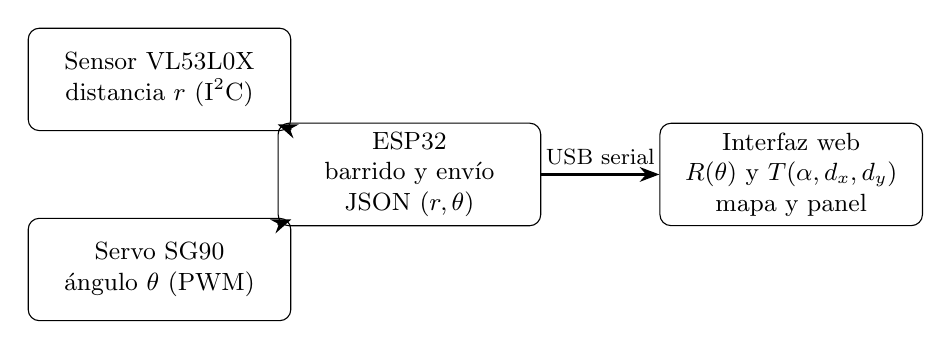
\begin{tikzpicture}[
  bloque/.style={draw, rounded corners, align=center, minimum height=1.3cm,
                 text width=3.1cm, font=\small},
  flecha/.style={-{Stealth[length=2.5mm]}, thick},
  node distance=1.1cm]
\node[bloque] (sensor) {Sensor VL53L0X\\ distancia $r$ (I\textsuperscript{2}C)};
\node[bloque, below=of sensor] (servo) {Servo SG90\\ ángulo $\theta$ (PWM)};
\node[bloque, right=1.5cm of $(sensor)!0.5!(servo)$] (esp) {ESP32\\ barrido y envío\\ JSON $(r,\theta)$};
\node[bloque, right=1.5cm of esp] (web) {Interfaz web\\ $R(\theta)$ y $T(\alpha,d_x,d_y)$\\ mapa y panel};
\draw[flecha] (sensor) -- (esp);
\draw[flecha] (esp) -- (servo);
\draw[flecha] (esp) -- node[above, font=\footnotesize]{USB serial} (web);
\end{tikzpicture}
\end{document}
